% XeLaTeX can use any Mac OS X font. See the setromanfont command below.
% Input to XeLaTeX is full Unicode, so Unicode characters can be typed directly into the source.

% The next lines tell TeXShop to typeset with xelatex, and to open and save the source with Unicode encoding.

%!TEX TS-program = xelatex
%!TEX encoding = UTF-8 Unicode

\documentclass[11pt]{article}
\usepackage{geometry,authblk,multicol,amsmath}
\usepackage[square,numbers,sort&compress]{natbib}
\usepackage[textsize=small]{todonotes}                % See geometry.pdf to learn the layout options. There are lots.
\geometry{letterpaper}                   % ... or a4paper or a5paper or ... 
%\geometry{landscape}                % Activate for for rotated page geometry
%\usepackage[parfill]{parskip}    % Activate to begin paragraphs with an empty line rather than an indent
\usepackage{graphicx}
\usepackage{amssymb}

% Will Robertson's fontspec.sty can be used to simplify font choices.
% To experiment, open /Applications/Font Book to examine the fonts provided on Mac OS X,
% and change "Hoefler Text" to any of these choices.

\usepackage{fontspec,xltxtra,xunicode}
\defaultfontfeatures{Mapping=tex-text}
\setromanfont[Mapping=tex-text]{Times New Roman}
\setsansfont[Scale=MatchLowercase,Mapping=tex-text]{Gill Sans}
\setmonofont[Scale=MatchLowercase]{Andale Mono}

\title{Mixture Models for Single Cell Assays}
\author[1]{Greg Finak}
\author[1]{\ldots Others \ldots}
\author[1]{Raphael Gottardo}

\affil[1]{Vaccine and Infectious Disease Division, Fred Hutchinson Cancer Research Center (FHCRC), Seattle, WA}
\date{\today}                                       

\begin{document}
\maketitle
\begin{abstract}
Immunological endpoints in vaccine trials are measured through a number of different assays that often provide single--cell measurements of multiple, specific intracellular or cell surface proteins, or mRNA expression levels of genes in single cells from specific cell sub--populations. While these measurements are continuous, they are generally discretized during data analysis. For example, in flow cytometry, individual cells are often classified as either positive or negative for a marker based on a predetermined threshold.  One such assay is the intracellular cytokine staining assay that is used to assess an individual's immune response to a vaccine by measuring the abundance antigen--specific T--cell subpopulations producing different cytokines. Cells are classified as cytokine positive or negative based on some threshold, and the resulting discretized count data is used to test for an increase in cytokine producing cells between a treatment and control sample. ICS assays are generally used to identify ``vaccine responders''. These are individuals whose immune system produces significantly more cytokine positive cells in response to antigen stimulation than at baseline. The rarity of these cell populations makes maximizing the sensitivity and specificity of the assay a primary concern. The typical approach to analysis using Fisher's exact test is problematic for two reasons. It can be overly conservative in detecting true differences for small counts, and the data generally do not meet the assumptions of the test. Specifically, the total cell counts across conditions are generally not fixed since these are generated by independent experiments.  In this paper we present a cohort framework based on an empirical-Bayes mixture of Beta--binomial or Dirichlet--Multinomial distributions, for analyzing count data derived from such thresholded single--cell assays. In general, any single--cell assay in which continuous data can be thresholded to classify individual cells into either ``positive'' or ``negative'' categories with respect to one or more variables and compared across different conditions, is suitable for analysis using our method and the extensions presented herein. Using the ICS assay as a motivating example, our method models cytokine–specific T-cell response across all individuals simultaneously while modelling the stimulated and unstimulated cell counts independently. Using simulations and real--world vaccine trial data, we show that our model increases the sensitivity and specificity for positivity calls in ICS assays compared to Fisher's exact test.
\end{abstract}

\section{Introduction}
Single--cell assays are an important tool in immunology, providing a functional and phenotypic snapshot of the immune system at a given time. These assays typically measure multiple variables simultaneously on individual cells in a homogeneous mixture such as whole blood. These variables are used to classify individual cells in the mixture into more homogeneous sub populations based on phenotypic or functional differences. Such single--cell assays provide a snapshot of immune function at a given time and are used for immune monitoring of disease, vaccine research, and diagnosis of haematological malignancies~\cite{}.  

A motivating example from vaccine trial research is the flow cytometric intracellular cytokine staining (ICS) assay, which is used to identify individuals whose immune system responds to a vaccine. Upon vaccination, antigen in the vaccine is taken up and presented to CD4 or CD8 T--cels via antigen presenting cells. Not all T--cells can recognize all antigens. Those that recognize antigens in the vaccine become \emph{activated} and produce a variety of cytokines that further promote the immune response. After activation, this antigen--specific subpopulation proliferates and can persist in the immune system for some time providing \emph{memory} that can more rapidly recognize the same antigen again in the future. None the less, these antigen--specific T--cell subpopulations a very small fraction of the total number of CD4 and CD8 T--cells. The ICS assay measures the number of antigen--specific T--cells in whole blood by measuring cytokine production in response to activation following stimulation by an antigen that was present in the original vaccine. Individual cells are labelled using fluorescently conjugated antibodies against phenotypic markers (CD3, CD4, and CD8) and functional markers (cytokines) of the cell subpopulations of interest~\cite{Horton:2007tsa,DeRosa:2004wp,Betts:2006dw}. A sufficiently large number of cells must be collected to ensure that the rare cell populations can be detected. Subsequently, each individual cell is classified as either positive or negative for each maker based on predetermined thresholds, then the number of cells matching each subpopulation phenotype is counted. These counts are compared between antigen stimulated and unstimulated samples from an individual to identify significant differences. Assessing a broad T cell response to a vaccine is particularly important in HIV vaccine trials, where the search for immune correlates of protection against HIV progression and infection is ongoing~\cite{Plotkin:2010ve,Horton:2007tsa,Kim:2010fw}.

The ICS assay in flow cytometry is just one example of the applications of single--cell technologies to immunology. Single--cell gene expression technologies such as Fluidigm are enabling researchers to measure the expression of 96 genes in 96 single cells from a homogeneous population sorted by flow cytometry\cite{Jang:2011uj}. This technology has been used to identify signatures of immune cell sub--populations that correlate with different types of vaccine~\cite{Flatz:2011jb}.

\section{Materials and Methods}

\subsection{Vaccine Trial ICS Dataset Description}
HVTN054 is a phase 1 (safety and efficacy) trial of an adenoviral vector vaccine in individuals without prior immunity~\cite{Peiperl:2010ej}. The vaccine vector expressed Gag, Pol and Env proteins from multiple HIV clades~\cite{Peiperl:2010ej}. Vaccine was given at two increasing doses, as well as a placebo. T--cell responses to antigens in the vaccine were measured via the ICS assay~\cite{Peiperl:2010ej,Horton:2007tsa}. The cytokines measured were IFNg (Interferon--$\gamma$), IL2 (Interleukin--2), TNFa (Tumor necrosis factor--$\alpha$) and IL4 (Interleukin 4)~\cite{Horton:2007tsa}. The sample size consisted of 20 vaccine and four placebo recipients. Statistical analysis of the original positivity calls is described in the original publication~\cite{Peiperl:2010ej}.
 
 
\subsection{Data Import, Preprocessing, and Gating}
The gated ICS assay data was imported into R from the original flowJo workspaces (version 6, TreeStar Inc, Ashland, OR)  using the BioConductor tool, \textit{flowWorkspace} (v 1.1.6) and ncdfFlow (v 1.1.4). Data were preprocessed using the flowJo--defined compensation matrices and data transformations extracted from the workspace file, and gated using methods from the flowCore package (v 1.19.2) to extract counts of cytokine positive and negative T--cells for each sample and stimulation~\cite{Hahne:2009vv}.

\subsection{Statistical Analysis of Responder and Non--responder calls}
Below, we summarize the methods for statistical analysis of responder and non--responder calls in the published trial, as well as the methods compared in this paper.
\subsubsection{Statistical Analysis in the Published Trial}
The methodology for statistical analysis and calling responders and non--responders in the original vaccine trial is described in the original publication~\cite{Peiperl:2010ej}. In general, a participant is called a ``responder'' to an antigen stimulation if, for a given cytokine, the number of cytokine--positive T-cells in the antigen--stimulated sample is significantly greater (for some statistical measure of significance) than the number of cytokine--positive T-cells for the negative control (unstimulated) sample from the same individual. In the original trial, significance was measured via one--sided Fisher's exact test for each participant and cytokine, comparing stimulated against unstimulated samples from that individual. A discrete Bonferroni adjustment for multiple comparisons was applied, and stimulations with an adjusted p--value below $\alpha = 0.00001$ were called positive. 


\subsection{Statistical Analysis of Responder and Non--responder Calls for Direct Comparison Against the Bayesian Mixture Model Approach}
Positivity calls for vaccine responders and non--responders depend upon the selection of an appropriate threshold. Therefore, to compare different methods of analysis, comparable thresholds for positivity must be selected for the methods. Our mixture modelling approach is fit within each stimulation, and we make positivity calls based on a false discovery rate calculated across individuals, within each stimulation, whereas the originally published analysis makes multiple testing adjustments within individuals, across cytokines \todo[inline]{IS THIS CORRECT, OR IS IT WITHIN INDIVIDUALS ACROSS STIMULATIONS?}. In order to have comparable response rates, we reanalyzed the ICS data using Fisher's one--sided exact test (as described in the original publication) but made positivity calls based on the false discovery rate computed across individuals within each stimulation.

\subsection{Two Competing Beta--Binomial Models}
Our approach to modelling an individual's response to vaccine using ICS data takes a Bayesian approach. We model all observations (individuals) simultaneously for each combination of cytokine and stimulation (including the unstimulated samples). For a given cytokine, we let $n_s$ be the number of cytokine--positive cells in the stimulated sample, $N_s$ the total number of cells in the stimulated sample, and $n_u, N_u$, the number of cytokine--positive and total number of cells in the unstimulated sample, respectively. Note that usually, $N_u \ne N_s$. The observed count data $\mathbf{y}$ is a matrix of size $4 \times P$, where $P$ is the number of participants. For the $i$'th individual $\mathbf{y}_i = \left<N_{si},n_{si},N_{ui},n_{ui}\right>$, and can be represented as the following contingency table: 
% latex table generated in R 2.14.0 by xtable 1.5-6 package
% Wed Oct 12 09:41:50 2011
\begin{table}[ht]
\centering
\parbox{0.8\linewidth}{
\caption{2 x 2 contingency table of counts for cytokine positive and cytokine negative events between stimulated and unstimulated conditions}\label{tab:twobytwo}
\centering
\begin{tabular}{rrr}

  \hline
\multicolumn{1}{l}{}&
\multicolumn{2}{c}{Cytokine}\\
 & Negative & Positive \\ 
  \hline
Stimulated &   $N_{si} - n_{si}$ &   $n_{si}$ \\ 
Unstimulated &   $N_{ui}-n_{ui}$ &   $n_{ui}$ \\ 
   \hline
\end{tabular}
}
\end{table}

The positive cell counts for stimulated and unstimulated samples from the same individual are modelled as:
\begin{align}
  \text{if }&p_{si}=p_{ui}\equiv p_{0i};& n_{si} \sim \mathrm{Bin}(N_{si},p_u);\text{ }& n_{ui} \sim \mathrm{Bin}(N_{ui},p_{ui})\label{eq:null}\\
 \text{if }&p_{si}>p_{ui};& n_{si} \sim \mathrm{Bin}(N_{si},p_{si});\text{ }& n_{ui} \sim \mathrm{Bin}(N_{ui},p_{ui})\label{eq:alternate}
 \end{align}
Where $p_{si}$ and $p_{ui}$ are the unobserved proportions. Equation~\eqref{eq:null} represents the \textit{null} hypothesis where there is no difference between the stimulation and the control. Equation~\eqref{eq:alternate} represents the  alternate hypothesis where the cytokine response is stronger in the stimulation than in the control. We place a common Beta prior on the $p_{si}$ and $p_{ui}$ across individuals, as shown:
 
 \begin{align}
 p_{si} &\sim \mathrm{Beta}(\alpha_s,\beta_s)\label{eq:stimprior}\\
 p_{ui} &\sim \mathrm{Beta}(\alpha_u, \beta_u)\label{eq:nullprior}
 \end{align}
If $p_{si}=p_{ui}$ we assume that $\alpha_s=\alpha_u$ and $\beta_s=\beta_u$, thus sharing the hyper--parameters between the null and alternative model for the unstimulated samples, such that $\beta_u,\alpha_u$ hyper--parameters are equal for both the stimulated and unstimulated models. Given this formulation, the posterior probability of the data given that it is generated by model \eqref{eq:null}, is:
 \begin{align}
  	\mathrm{Pr}(y_i|\alpha_u,\beta_u)
	&=\binom{N_{si}}{n_{si}}\binom{N_{ui}}{n_{ui}}\frac{\mathrm{B}(n_{si}+n_{ui}+\alpha_u,N_{si}-n_{si}+N_{ui}-n_{ui}+\beta_u)}{\mathrm{B}(\alpha_u,\beta_u)}\label{eq:model1post}\\
	\intertext{with marginal log--likelihood:}
	\begin{split}
	\mathcal{L}(\alpha_u,\beta_u|\mathbf{y})=\sum_{i=1}^P\left[\log{\binom{N_{si}}{n_{si}}}+\log{\binom{N_{ui}}{n_{ui}}}+\right.\\
	\left.\log{\left(\mathrm{B}(n_{si}+n_{ui}+\alpha_u,N_{si}-n_{si}+N_{ui}-n_{ui}+\beta_u)\right)}\right]-P\log\left(\mathrm{B}(\alpha_u,\beta_u)\right)\label{eq:model1MLL}
	\end{split}
 \end{align} 
Thus, in the case of no response to stimulation, the counts for the stimulated and unstimulated samples are modelled as draws from the same "unstimulated" Beta--binomial distribution. Note that the unobserved parameters, $p_{si}, p_{ui}$ have been integrated out to give the marginal log--likelihood.


If the data is generated by model~\eqref{eq:alternate}, the posterior probability of the data is given by:
\begin{align}
	\begin{split}
\mathrm{Pr}(y_i|\alpha_u,\beta_u,\alpha_s,\beta_s) =\binom{N_{ui}}{n_{ui}} \binom{N_{si}}{n_{si}}\frac{\mathrm{B}(n_{ui}+\alpha_u,N_{ui}-n_{ui}+\beta_u)}{\mathrm{B}(\alpha_u,\beta_u)}\frac{\mathrm{B}(n_{si}+\alpha_s,N_{si}-n_{si}+\beta_s)}{\mathrm{B}(\alpha_s,\beta_s)}\cdot\\
	 \frac{\int\limits_{p_{ui}=0}\limits^{1}\left(\frac{1}{\mathrm{B}(n_{ui}+\alpha_u,N_{ui}-n_{ui}+\beta_u)}p_{ui}^{n_{ui}+\alpha_u-1}(1-p_{ui})^{N_{ui}-n_{ui}+\beta_u-1} \right)\left(\mathrm{I_{1-p_{ui}}}(N^i_s-n^i_s+\beta_s,n^i_s+\alpha_s)\right)d p_{ui}}{   \int\limits_{p_{ui}=0}\limits^{1}\left(\frac{1}{\mathrm{B}(\alpha_u,\beta_u)}p_{ui}^{\alpha_u-1}(1-p_{ui})^{\beta_u-1} \right)\left(\mathrm{I_{1-p_{ui}}}(\beta_s,\alpha_s)\right)d p_{ui}}
\label{eq:model2post}
\end{split}
	\intertext{with marginal log--likelihood:}
\begin{split}
\mathcal{L}(\alpha_s,\alpha_u,\beta_s,\beta_u|\mathbf{y})=-P\log\left(\mathrm{B}(\alpha_u,\beta_u)\right)-P\log\left(\mathrm{B}(\alpha_s,\beta_s)\right)+\\ \sum_{i=0}^P\left\{\log\binom{N_{ui}}{n_{ui}}+ \log\binom{N_{si}}{n_{si}}+ \log\left(\mathrm{B}(n_{ui}+\alpha_u,N_{ui}-n_{ui}+\beta_u)\right)+\right. \\ \left. \log\left(\mathrm{B}(n_{si}+\alpha_s,N_{si}-n_{si}+\beta_s)\right) + \right. \\ \left. \log\left[\hspace{1em}\int\limits_{p_{ui}=0}\limits^{1}\left(\frac{1}{\mathrm{B}(n_{ui}+\alpha_u,N_{ui}-n_{ui}+\beta_u)}p_{ui}^{n_{ui}+\alpha_u-1}(1-p_{ui})^{N_{ui}-n_{ui}+\beta_u-1} \right) \right. \right. \\  \left.\vphantom{\int\left( \frac{1}{\mathrm{B}(\alpha,\beta)}\right)}\left(\mathrm{I_{1-p_{ui}}}(N_{si}-n_{si}+\beta_s,n_{si}+\alpha_s)\right)d p_{ui}\right] \\ -  \left. \log\left[\hspace{1em}\int\limits_{p_{ui}=0}\limits^{1}\left(\frac{1}{\mathrm{B}(\alpha_u,\beta_u)}p_{ui}^{\alpha_u-1}(1-p_{ui})^{\beta_u-1} \right) \right. \right. \\  \left. \left.\vphantom{\int\left( \frac{1}{\mathrm{B}(\alpha,\beta)}\right)} \left(\mathrm{I_{1-p_{ui}}}(\beta_s,\alpha_s)\right)d p_{ui}\right] \right\}\label{eq:model2MLL}
\end{split}
\end{align}

The ratio of integrals in \eqref{eq:model2post} accounts for the different normalizing constants due to the constraints $p_{si}>p_{ui}$ on the prior and the posterior distributions. We call this the \emph{constrained} model. 

The term $I_{1-p_{ui}}(\beta_s,\alpha_s)=1-I_{p_{ui}}(\alpha_s,\beta_s)=Pr(p_{si} > p_{ui}; \alpha_s,\beta_s)$, is just the CDF of Beta distribution with parameters $\alpha_s,\beta_s$, leaving a 1--dimensional integration for the ratio of normalizing constants.

Without constraints, ($p_s\ne p_u$), the ratio of integrals for the normalizing constant in \eqref{eq:model2post} is dropped. We call this the \emph{unconstrained} model.


\subsection{The Mixture of Beta--Binomials}
Although we have specified the two models for the data, we do not know which observation was generated by which model. Clearly, not all individuals are expected to exhibit an immune response to a stimulation. Any individual observation, $y_i$, could either be generated by model~\eqref{eq:null} or by model~\eqref{eq:alternate}. We capture this uncertainty with a mixture framework of the two competing beta--binomial models. The likelihood for the mixture is given by:
\begin{align}
\begin{split}
%L(\alpha_s,\beta_s,\alpha_u,\beta_u,\pi_k|\mathbf{y})=\prod\limits_{i=1}\limits^P\left[ \pi_1 Pr(y_i|\alpha_u,\beta_u) +\pi_2 Pr(y_i|\alpha_u,\beta_u,\alpha_s,\beta_s) \right] ,\\ \sum\limits_{k=1}\limits^2\pi_k=1\\
L(\alpha_s,\beta_s,\alpha_u,\beta_u,\pi_k|\mathbf{y})=\prod\limits_{i=1}\limits^P\left[ \pi_1 f_1(y_i|\theta_1) +\pi_2 f_2(y_i|\theta_2) \right] ,\\ \sum\limits_{k=1}\limits^2\pi_k=1
\end{split}
\end{align}
Where $\theta_1=\{\alpha_u,\beta_u\}, \theta_2=\{\alpha_u,\beta_u,\alpha_s,\beta_s\}$, $\pi_1$ is the fraction of observations exhibiting no response to stimulation, $\pi_2$ the fraction of observations exhibiting a response to stimulation, and $f_1 = Pr(y_i|\alpha_u,\beta_u), f_2 = Pr(y_i|\alpha_u,\beta_u,\alpha_s,\beta_s)$ from \eqref{eq:model1post} and \eqref{eq:model2post}, above. 

The unobserved component memberships are treated as missing data and modelled as random variables  $\mathbf{z}_i = \left\{z_{i1},(1-z_{i1})\right\}$

$$
z_{ik} = \left\{ \begin{array}{rl}
1 &\mbox{ if observation $i$ is from the $k$'th model (component)} \\
0&\mbox{ otherwise}
\end{array} \right.
$$

Each $\mathbf{z}_{i}$ follows an independent multinomial distribution with one trial and  parameters $\boldsymbol{\pi}=\left\{\pi_1,1-\pi_1\right\}$. Given the $z_i$'s, the complete data log--likelihood is:

\begin{align}
\begin{split}
\mathcal{L}_c(\alpha_s,\beta_s,\alpha_u,\beta_u,\pi_k|\mathbf{y},\mathbf{z})=\sum\limits_{i=1}\limits^P\sum\limits_{k=1}\limits^2{z_{ik}\left[ \log\pi_k+\log f_k(y_i|\theta_k)\right]}\label{eq:CDLL}
\end{split}
\end{align}

In this form, we use the expectation--maximization (EM) algorithm~\cite{Dempster:1977ul} to fit the model. 

\subsubsection*{E--step}
Given the model parameters $\boldsymbol{\Psi}=\left\{\alpha_u,\beta_u,\alpha_s,\beta_s,\pi_k\right\}$, and the data $\mathbf{y}$, we estimate the unobserved component memberships, $\mathbf{Z_i}$  by computing the conditional expectation of the $\mathbf{Z_i}$'s,  $\mathbb{E}\boldsymbol{_\Psi}(\mathbf{Z_i}|\mathbf{y}_i)$:
\begin{align}
\tilde z_{ik} &= \frac{\pi_k f_k(\mathbf{y}_i|\theta_k)}{\sum\limits_{k=1}\limits^{2}\pi_kf_k(\mathbf{y}_i|\theta_k)}
\end{align}

\subsubsection*{M--step}
Finally, given the $\tilde{z}_{ik}$, we update the estimates of the model parameters to maximize the conditional expectation of the complete--data log--likelihood. The mixing proportions are given by:
\begin{align}
\hat\pi_k = \frac{ \sum_i^P \tilde z_{ik}}{n}
\end{align}

There is no closed form for the model hyper--parameters, $\alpha_u,\beta_u,\alpha_s,\beta_s$, and they are estimated via numerical optimization using R's \textit{optim} function. For this purpose they are re--parameterized as $\mu_u=\frac{\alpha_u}{\alpha_u+\beta_u}$ and $S=\alpha_u+\beta_u$ (likewise for the $\alpha_s,\beta_s$), corresponding to the mean and sample size of the prior distributions. 

\subsubsection*{Initialization}
We initialize the $z_{ik}$'s using Fisher's exact test to assign each observation to either the $p_{si}=p_{ui}$ or $p_{si} > p_{ui}$ components. We then use the $\hat{z}_i$'s to initialize the hyper--parameters to their method--of--moments estimates:
\begin{align}
\hat{\alpha} = \hat{\mu}\left(\frac{\hat{\mu}(1-\hat{\mu})}{\hat{\sigma}^2} -1\right)\\
\hat{\beta} =  (1-\hat{\mu}\left(\frac{\hat{\mu}(1-\hat{\mu})}{\hat{\sigma}^2} -1\right)
\end{align}

Where $\hat{\mu}$ and $\hat{\sigma}^2$ are the sample mean and sample variance estimates, given the $z_{ik}$'s.

\subsection*{Generalization to Multiple Cytokines and Polyfunctionality with the Multinomial Dirichlet}
The model can be generalized to handle multiple cytokines in a single stimulation, in order to assess polyfunctional cytokine responses of T--cells. We use the Multinomial--Dirichlet family of distributions to model counts of events in two \textit{different} 2x2 contingency tables. Here we consider only the \emph{unconstrained} case ($p_s\ne p_u$). The observed data can be represented in the following way: 

\begin{table}[ht]
\centering
\parbox{0.8\linewidth}{
\caption{Contingency tables for counts of cells expressing two cytokines between stimulated and unstimulated conditions. $n_{\{s,u\}j}$ denotes observed counts for stimulated or unstimulated table cell $j$, and individual $i$  }\label{tab:multdir}
\begin{minipage}[b]{0.5\linewidth}
\centering
\begin{tabular}{rrr}
\multicolumn{3}{c}{Stimulated}\\
  \hline
\multicolumn{1}{l}{}&
\multicolumn{2}{c}{Cytokine A}\\
 & Negative & Positive \\ 
 \multicolumn{1}{l}{Cytokine B}&&\\
  \hline
Negative &   $n_{si1}$ &   $n_{si2}$ \\ 
Positive &   $n_{si3}$ &   $n_{si4}$ \\ 
   \hline
\end{tabular}
\end{minipage}
\begin{minipage}[b]{0.5\linewidth}
\centering
\begin{tabular}{rrr}
\multicolumn{3}{c}{Unstimulated}\\
  \hline
\multicolumn{1}{l}{}&
\multicolumn{2}{c}{Cytokine A}\\
 & Negative & Positive \\ 
 \multicolumn{1}{l}{Cytokine B}&&\\
  \hline
Negative &   $n_{ui1}$ &   $n_{ui2}$ \\ 
Positive &   $n_{ui3}$ &   $n_{ui4}$ \\ 
   \hline
\end{tabular}
\end{minipage}
}
\end{table}

Where the vector of observed counts for individual $i$ in the stimulated or unstimulated sample is denoted: $\bar{n}_{\{s,u\}i} = \{n_{\{s,u\}ij}\} ; j\in\{1\ldots 4\}$, and $j$ indexes the cells of the appropriate contingency table shown in~Table~\ref{tab:multdir}. The counts are modelled as draws from different multinomial distributions:
\begin{align}
\text{if } & \bar{p}_{si}=\bar{p}_{ui};& \bar{n}_{ui} \sim \mathcal{M}(\bar{p}_{ui},N_{ui});\bar{n}_{si} \sim \mathcal{M}(\bar{p}_{ui},N_{si})\\
\text{if } & \bar{p}_{si} \ne \bar{p}_{ui};& \bar{n}_{ui} \sim \mathcal{M}(\bar{p}_{ui},N_{ui});\bar{n}_{si} \sim \mathcal{M}(\bar{p}_{si},N_{si})
\end{align}
with Dirichlet priors on the proportions:
\begin{align}
\bar{p}_{si} \sim \mathrm{Dir}(\bar{\alpha}_s) ; \bar{p}_{ui} \sim \mathrm{Dir}(\bar{\alpha}_u)
\end{align}

For the null component, where $\bar{p}_{s}=\bar{p}_{u}$ the marginal likelihood is given by: 
\begin{align}
\mathrm{L}(\bar{n}_s,\bar{n}_u,N_s,N_u|\bar{\alpha}_u) &= \prod_{i=0}^P\frac{ \mathrm{B_j}(\bar{\alpha}_{u}+\bar{n}_{ui}+\bar{n}_{si})}{\mathrm{B_j}(\bar{\alpha}_u)} \cdot \frac{N_{si}!}{\prod_{j=1}^J n_{sij}!} \cdot \frac{N_{ui}!}{\prod_{j=1}^J n_{uij}!}\label{NRmd}
\end{align}
Where $\mathrm{B_j}$ is the $\mathrm{j}$--dimensional Beta function: $\frac{\prod_{j=1}^J\Gamma(\alpha_j)}{\Gamma(\sum\alpha_j)}$.

The marginal likelihood for a component where $p_{sj} \ne p_{uj}$ for all $j$, is given by:
\begin{align}
\mathrm{L}(\bar{n}_s,\bar{n}_u,N_s,N_u|\bar{\alpha}_u,\bar{\alpha}_s) &= \prod_{i=0}^P\frac{  \mathrm{B_j}(\bar{\alpha}_{u}+\bar{n}_{ui}) \mathrm{B_j}(\bar{\alpha}_{s}+\bar{n}_{si})}{\mathrm{B_j}(\bar{\alpha}_s)\mathrm{B_j}(\bar{\alpha}_u)} \cdot \frac{N_{si}!}{\prod_{j=1}^J n_{sij}!} \cdot \frac{N_{ui}!}{\prod_{j=1}^J n_{uij}!}\label{eq:postmult}
\end{align}

Without loss of generality, if only some $p_j$ are different between stimulated and unstimulated samples, the appropriate components of $\alpha_j$  can be substituted in the calculation of the likelihood eq~\eqref{eq:postmult}.


The marginal likelihood of the non--responding component, given in eq~\eqref{NRmd} can be rewritten as:
\begin{align}
\begin{split}
l(\bar{\alpha}_u|D)=\sum_i \left[ \log \Gamma (\sum_j \alpha_{uj}) - \log \Gamma (\sum_j \alpha_{uj}+n_{uij}+n_{sij})+ \sum_j (\log \Gamma(\alpha_{uj}+n_{uij}+n_{sij}) \right.\\ \left. -\log\Gamma(\alpha_{uj}))+ \log\Gamma(N_{si}+1) +\log\Gamma(N_{ui}+1)-\right.\\ \left.\left[\sum_j(\log\Gamma(n_{sij}+1)+\log\Gamma(n_{uij}+1))\right]\right]\label{mdloglike}
\end{split}
\end{align}

The gradient is given by:
\begin{align}
\frac{\partial l}{ \partial \alpha_{uj}} = \sum_i \Psi(\sum_j \alpha_{uj}) - \Psi (\sum_j \alpha_{uj}+n_{uij}+n_{sij}) + \Psi(\alpha_{uj}+n_{uij}+n_{sij}) - \Psi(\alpha_{uj})\label{mdgrad}
\end{align}

and the Hessian is:
\begin{align}
j&\ne k; &\frac{\partial^2 l}{\partial \alpha_{uj}\alpha_{uk}} & = \sum_i \Psi'(\sum_j\alpha_{uj})-\Psi'(\sum_j\alpha_{uj}+n_{uij}+n_{sij})\\
j&=k;&\frac{\partial^2l}{\partial \alpha_{uj}^2} &= \sum_i \Psi'(\sum_j\alpha_{uj})-\Psi'(\sum_j\alpha_{uj}+n_{uij}+n_{sij})+\Psi'(\alpha_{uj}+n_{uij}+n_{sij})-\Psi'(\alpha_{uj})
\end{align}

The marginal likelihood of the responding component in eq~\ref{eq:postmult} can be rewritten as:
\begin{align}
\begin{split}
\sum_i\bigg[\sum_j \big[ \log\Gamma(\alpha_{uj}+n_{uij})+\log\Gamma(\alpha_{sj}+n_{sij}) -\log\Gamma(\alpha_{uj}) -\log\Gamma(\alpha_{sj})\\
-\log\Gamma(n_{sij}+1)-\log\Gamma(n_{uij}+1)\big]+\log\Gamma(\sum_j\alpha_{sj})+\log\Gamma(\sum_j\alpha_{uj})\\
-\log\Gamma(\sum_j\alpha_{uj}+n_{uij})-\log\Gamma(\sum_j\alpha_{sj}+n_{sij})+\log\Gamma(N_{si}+1)+\log\Gamma(N_{ui}+1)\bigg]
\end{split}
\end{align}
with gradient:
\begin{align}
\frac{\partial l}{\partial\alpha_{\phi j}} = \sum_i \Psi(\alpha_{\phi j}+n_{\phi ij})-\Psi(\alpha_{\phi j})+\Psi(\sum_j \alpha_{\phi j}) - \Psi(\sum_j \alpha_{\phi j}+n_{\phi ij}): (\phi \in {s,u})
\end{align}
and Hessian:
\begin{align}
\frac{\partial^2l}{\partial \alpha_{\phi j}^2}& \overset {k=j}{=}\sum_i \Psi'(\alpha_{\phi j}+n_{\phi ij}) - \Psi'(\alpha_{\phi j}) + \Psi'(\sum_j \alpha_{\phi j}) - \Psi'(\sum_j\alpha_{\phi j}+n_{\phi ij})\\
\frac{\partial^2l}{\partial \alpha_{\phi j}\alpha_{\phi k}}&\overset{k\ne j}{=}\sum_i\Psi'(\sum_j \alpha_{\phi j}) - \Psi'(\sum_j\alpha_{\phi j}+n_{\phi ij})
\end{align}

\subsubsection*{Mixture Model Complexity}
We may wish to detect any of $2^3 = 8$ different possible scenarios where the proportion of events in corresponding cells of the contingency tables are either equal or unequal between stimulated and unstimulated conditions. Such a model would have 8 components and 55 parameters. However, if we recognize that the models can be nested, i.e. that parameters can be shared across components with similar outcomes, then the number of parameters can be reduced to 19, and further to 15 if we only consider components where any one cell of the tables differs between stimulated and unstimulated conditions. This is outlined in Table~\ref{tab:nesting}.
\begin{table}
\centering
\parbox{0.8\linewidth}{\caption{Nesting of models and parameter counts. Each row is a model component. The three columns correspond to cells two, three, and four of the contingency tables shown in Table~\ref{tab:multdir}. An open circle at a position indicates that the component models $p_{sj}=p_{uj}$, and a filled circle indicates that the component models $p_{sj}\ne p_{uj}$. The number of additional parameters that need to be estimated by including each additional component in the mixture model is in the fourth column (number of parameters for proportions + number of parameters for component weights).}\label{tab:nesting}
\centering
\begin{tabular}{ccccc}
\multicolumn{3}{c}{Cell of Table}\\
\hline
cell 2&cell 3&cell 4&\# of parameters\\
\hline
$\circ$&$\circ$&$\circ$&6+1\\
$\circ$&$\circ$&$\bullet$&2+1\\
$\circ$&$\bullet$&$\circ$&2+1\\
$\bullet$&$\circ$&$\circ$&2+1\\
$\circ$&$\bullet$&$\bullet$&0+1\\
$\bullet$&$\bullet$&$\circ$&0+1\\
$\bullet$&$\circ$&$\bullet$&0+1\\
$\bullet$&$\bullet$&$\bullet$&0\\
\end{tabular}
}
\end{table}

\subsection*{Simulation Studies}
We examined the performance of the constrained ($p_s>p_u$) and unconstrained ($p_s \ne p_u$) beta--binomial mixture models via simulations. Using hyper parameters estimated from the model fit of the constrained model to data from Gag1 stimulated CD4--positive, IL2 expressing T--cells on day 28 from the HVTN054 data set, we simulated data from the constrained model with 500 observations, a response rate of 40\%, an $N$ of 10K, 20K, 30K, 50K, 75K, 100K, and 150K events, and ten independent realizations for each $N$. The constrained model was fit to this data and the sensitivity and specificity of the model's ability to correctly identify observations from the ``responder'' and ``non--responder'' components was evaluated through ROC curve analysis and compared against Fisher's exact test. (Figure~\ref{fig:simulations}). The nominal vs observed false discovery rate was also examined for the models and for Fisher's exact test, as well as the accuracy of the estimated prior distributions. In order to assess whether the unconstrained model could be used to effectively fit data from a constrained model and benefit from faster computations using exact closed form expressions rather than Monte-Carlo integration, we fit the same data simulated from the constrained model using the unconstrained model (Figure~\ref{fig:simulations}. 

To assess the sensitivity of the model to deviations from model assumptions, we repeated the simulations with the cell proportions drawn from  truncated normal distributions on $(0,1)$, rather than beta distributions. The means and variances of the truncated normal distributions were set to the MLE estimates of the beta distributions defined by the $\alpha,\beta$ hyper parameters estimated from the HVTN054 data set (Figure~\ref{fig:simulations_trunc}). 

\section*{Results}
\subsection*{Simulations Show MIMOSA Outperforms Fisher's Exact Test Event When Model Assumptions are Violated}
We ran simulation studies to assess the performance of the constrained and unconstrained models, as described in the Methods. We found that the both the constrained and unconstrained MIMOSA models out--performed Fisher's exact test with respect to sensitivity and specificity at all values of $N$, and that the false discovery rate observed for the mixture model more closely reflected the nominal false discovery rate than Fisher's exact test (Figure~\ref{fig:simulations}). Furthermore, both models gave reasonable estimates of the true hyper--parameters (Figure~\ref{fig:simulations}).

Since the constrained model relies on Monte--Carlo integration, which can be computationally costly, to estimate the normalizing constant in the likelihood calculation, we examined whether the unconstrained model could be used to accurately fit data generated from the constrained model. We found that the unconstrained model performed as well as the constrained model when fitting data generated from the constrained model (Figure~\ref{fig:simulations}).

In order to assess the sensitivity of the model to deviations from model assumptions, we fit the unconstrained model to simulated data where the proportions were drawn from truncated normal distributions (Figure~\ref{fig:simulations_trunc}). Even in these circumstances the unconstrained MIMOSA model outperformed Fisher's exact test and in fact performed about as well as the constrained model fit to constrained data.


\subsection*{MIMOSA Outperforms Fisher's Exact Test in Real--World Vaccine Trial Data from HVTN054}

We tested our method on ICS data from HVTN054, a safety and immunogenicity vaccine trial for a replication defective Adenovirus vector HIV vaccine. The data set consisted of 48 individuals who received two doses of vaccine or placebo, and ICS time points for these individuals were available at day 0 and day 28 after vaccination. Responders for each cytokine and stimulation combination were classified using Fisher's exact test and the constrained MIMOSA model at the 1\% FDR level, then the response rate within the control and treatment groups were calculated for both methods. Figure~\ref{fig:positivityrates} shows the response rates for a subset of the ICS data (Gag2 and Pol2 stimulations, for the IL2 and IFNg cytokines, at days 0 and 28, in both CD4 and CD8 T--cell subpopulations). On day 0, we found that the response rates from the MIMOSA model were zero, and equal to response rates computed from Fisher's exact test across all treatment and control groups. The same was true for the response rate in the control groups at day 28. In the treatment groups, at day 28, the response rates for the MIMOSA model were  generally higher or equal to those for Fisher's exact test, demonstrating the increased sensitivity and specificity of our method.

The MIMOSA framework generates predictions for individual samples. To better understand the differences between the predictions from the MIMOSA model and Fisher's exact test, we examined the model fit from Gag2 stimulated CD4+ T--cells at day 28 producing IFNg (Figure~\ref{fig:icsdata}). We see that two individuals are predicted as responders by the MIMOSA model which are not detected by Fisher's exact test. Both individuals have a larger proportion of IFNg producing antigen specific T--cells in antigen stimulated than unstimulated samples, as measure by the MAP or ML estimates of the proportions (Figure~\ref{fig:icsdata}). 

\begin{figure}[htbp] %  figure placement: here, top, bottom, or page
   \centering
   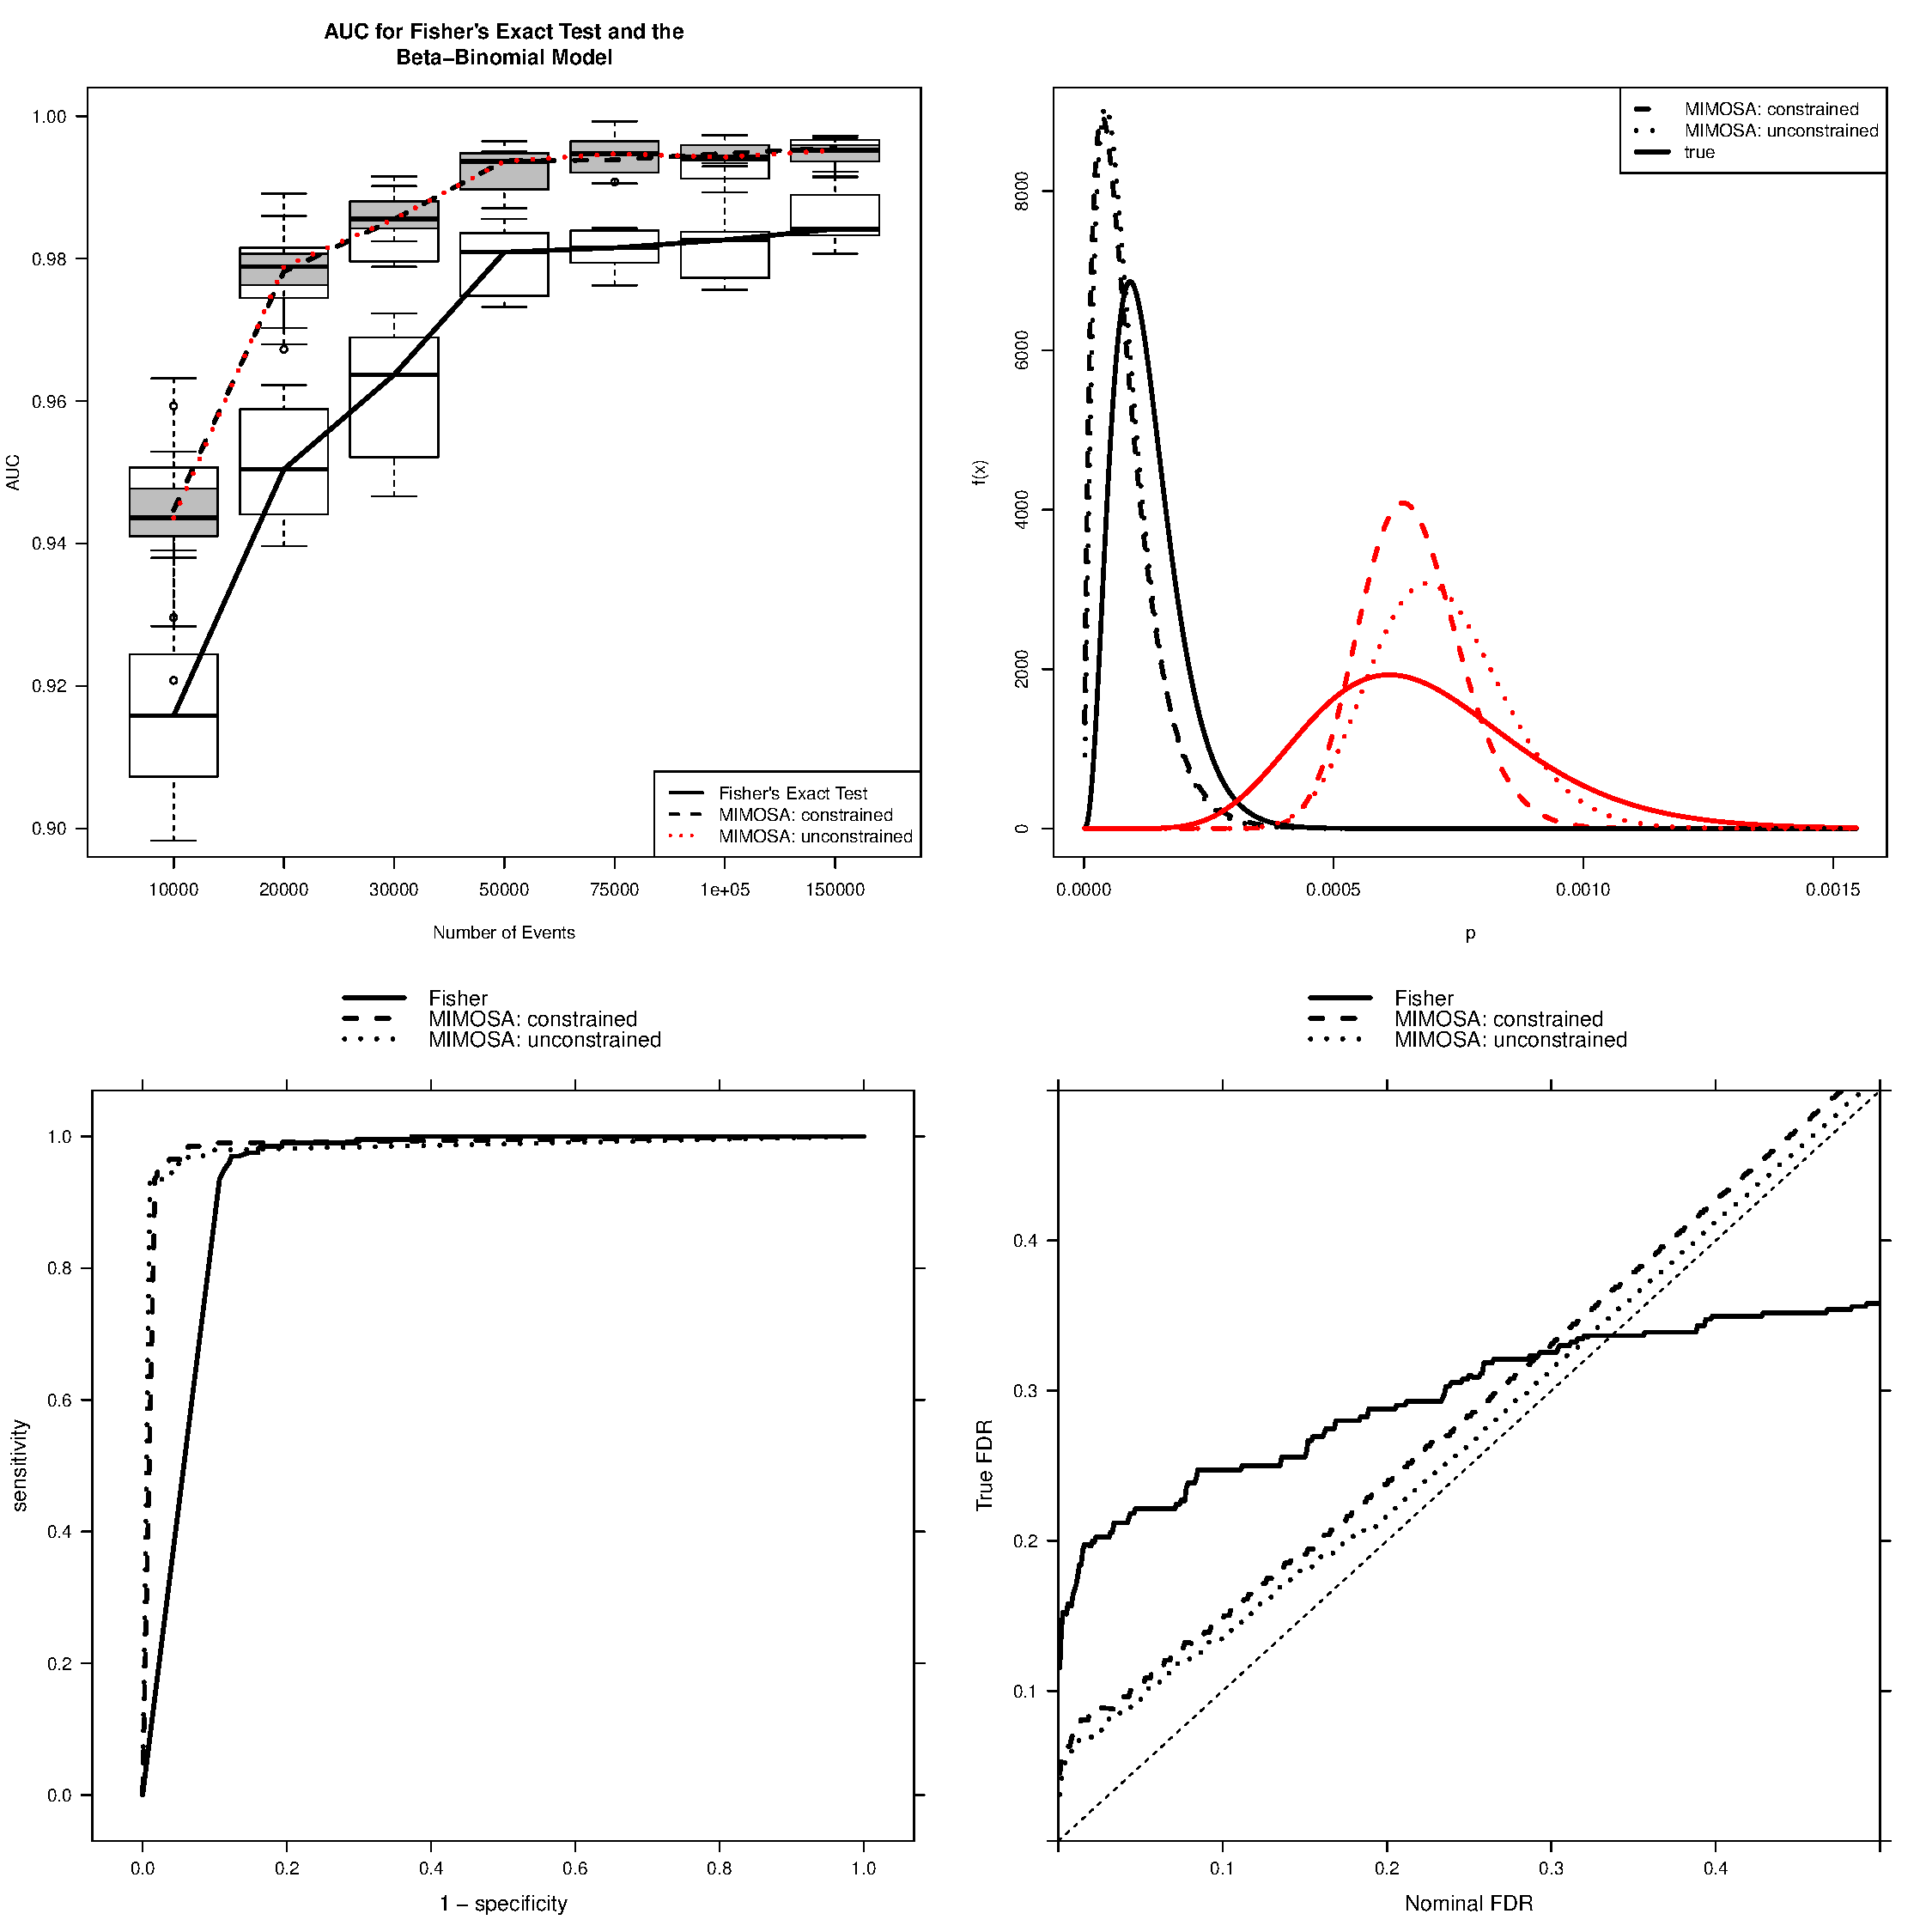
\includegraphics[width=4in]{Figures/simulations_all} 
   \caption{Performance of the constrained and unconstrained Beta--binomial mixture model vs Fisher's exact test on simulated data. Data were simulated from a constrained model with hyper--parameters estimated from a real data set of Gag1 stimulated, CD4+, IL2 expressing T--cells on day 28 from the HVTN054 trial. For total cell counts from 10,000 to 150,000, we simulated ten data sets each of 500 observations with a response rate of 40\%. The performance, measured by the AUC (area under the curve), of the constrained and unconstrained Beta--binomial mixture model compared to Fisher's exact test is shown in the first panel, as a function of increasing number of cells. The beta distributions for the estimated and true hyper parameters are shown in the second panel for one simulated data set, with N=150,000 events. The ROC curve for Fisher's exact test and the constrained and unconstrained Beta--binomial model for the same simulation are shown in the third panel. The observed vs expected false discovery rate for Fisher's exact test and the constrained and unconstrained Beta--binomial model are shown in the fourth panel.}
   \label{fig:simulations}
\end{figure}

\begin{figure}[htbp] %  figure placement: here, top, bottom, or page
   \centering
   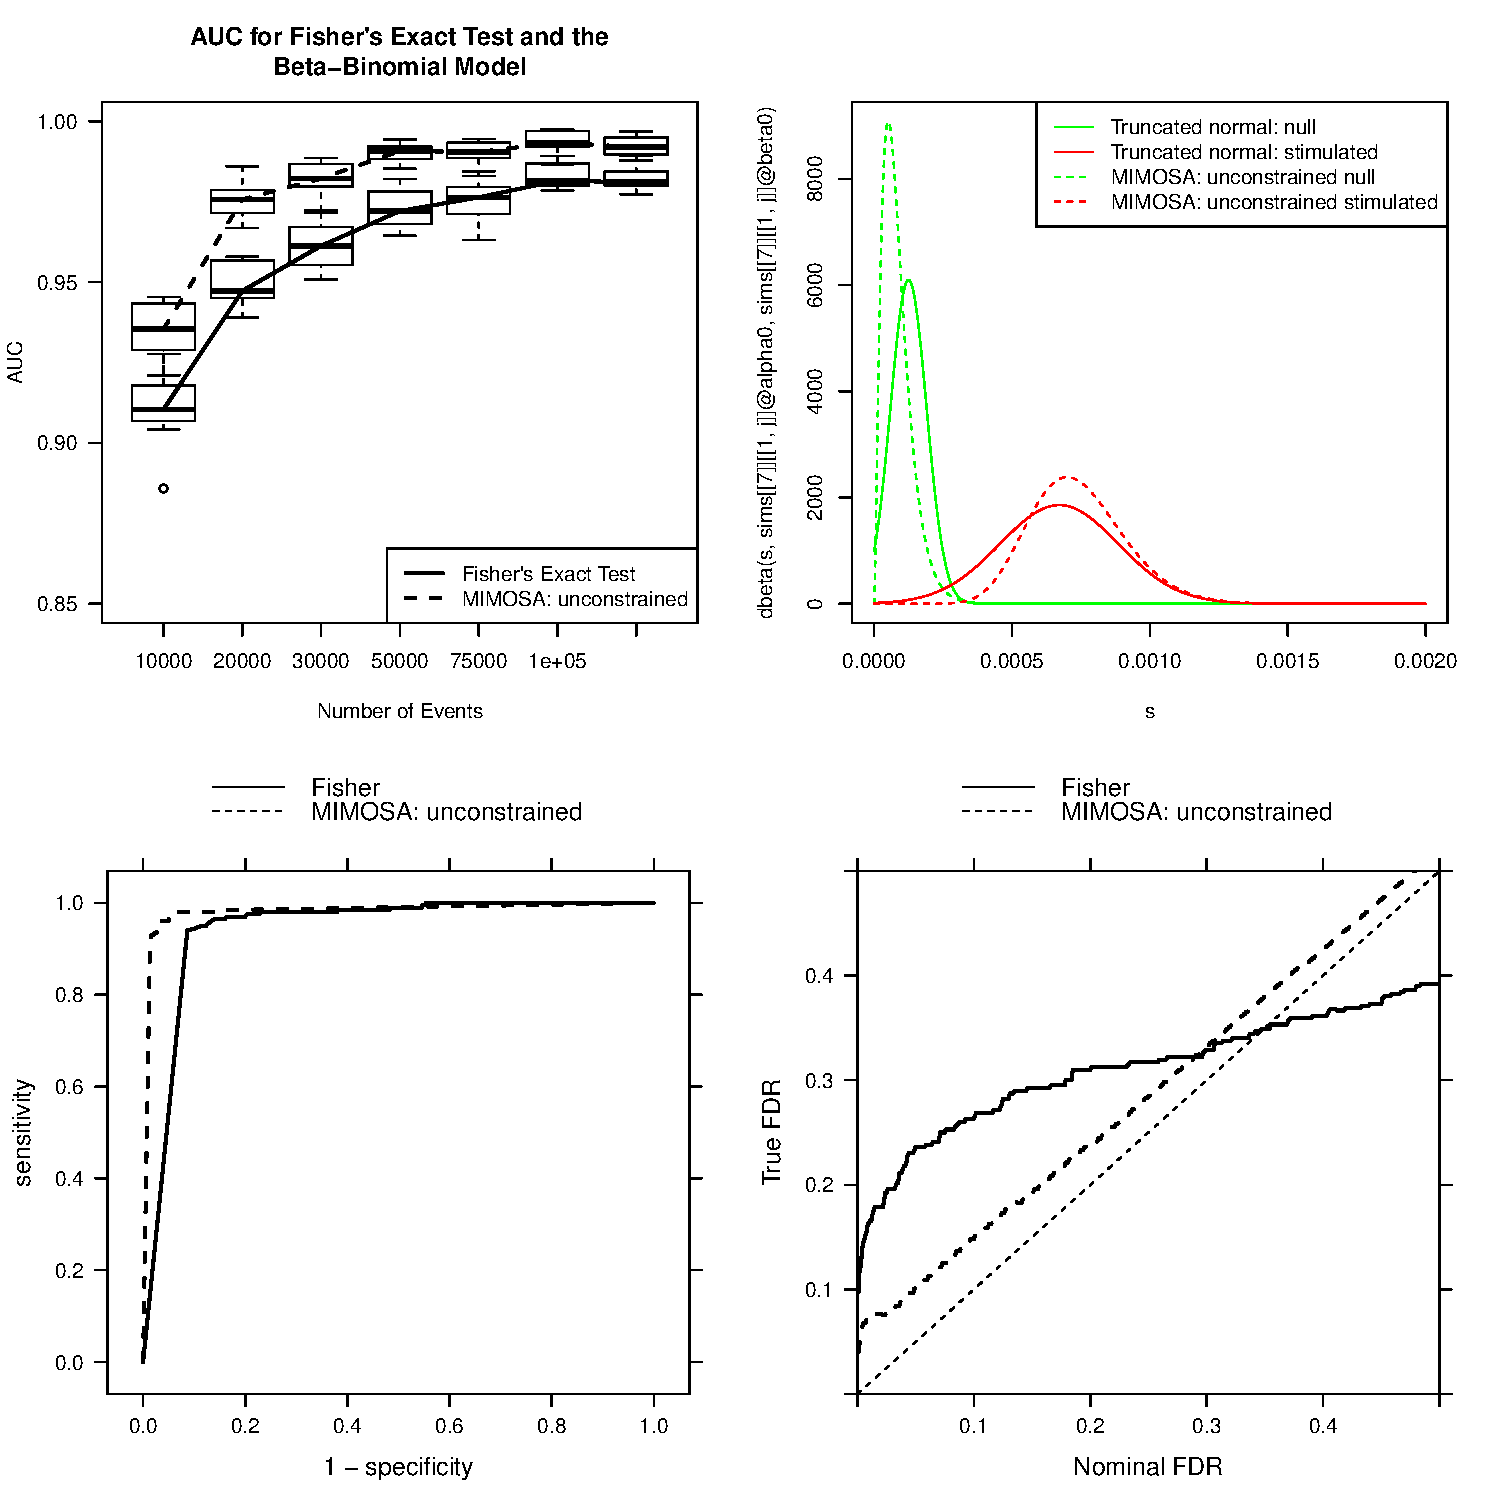
\includegraphics[width=4in]{Figures/simulations_violatedmodel} 
   \caption{Sensitivity to departures from model assumptions. We generated data from variant of the constrained model ($p_s>p_u$) where the proportions were simulated from truncated normal distributions on $(0,1)$, rather than from beta distributions. The mean and variance of the normal distributions was given by $\mu=\alpha/(\alpha+beta), \sigma^2=(\alpha\beta)/((\alpha+beta)^2(\alpha+\beta+1))$, where $\alpha,\beta$ are the Beta--prior hyper parameters for the MIMOSA model estimated from real data ($s, u$ subscripts omitted for brevity). The AUC for the unconstrained MIMOSA model and Fisher's exact test as a function of event count are shown in the first panel. The beta distributions for the estimated and true hyper parameters  are shown in the second panel. The ROC curves for one data set and the observed and true false discovery rates for the model and Fisher's exact test are shown in the third and fourth panels.}
   \label{fig:simulations_trunc}
\end{figure}


\begin{figure}[htbp] %  figure placement: here, top, bottom, or page
   \centering
   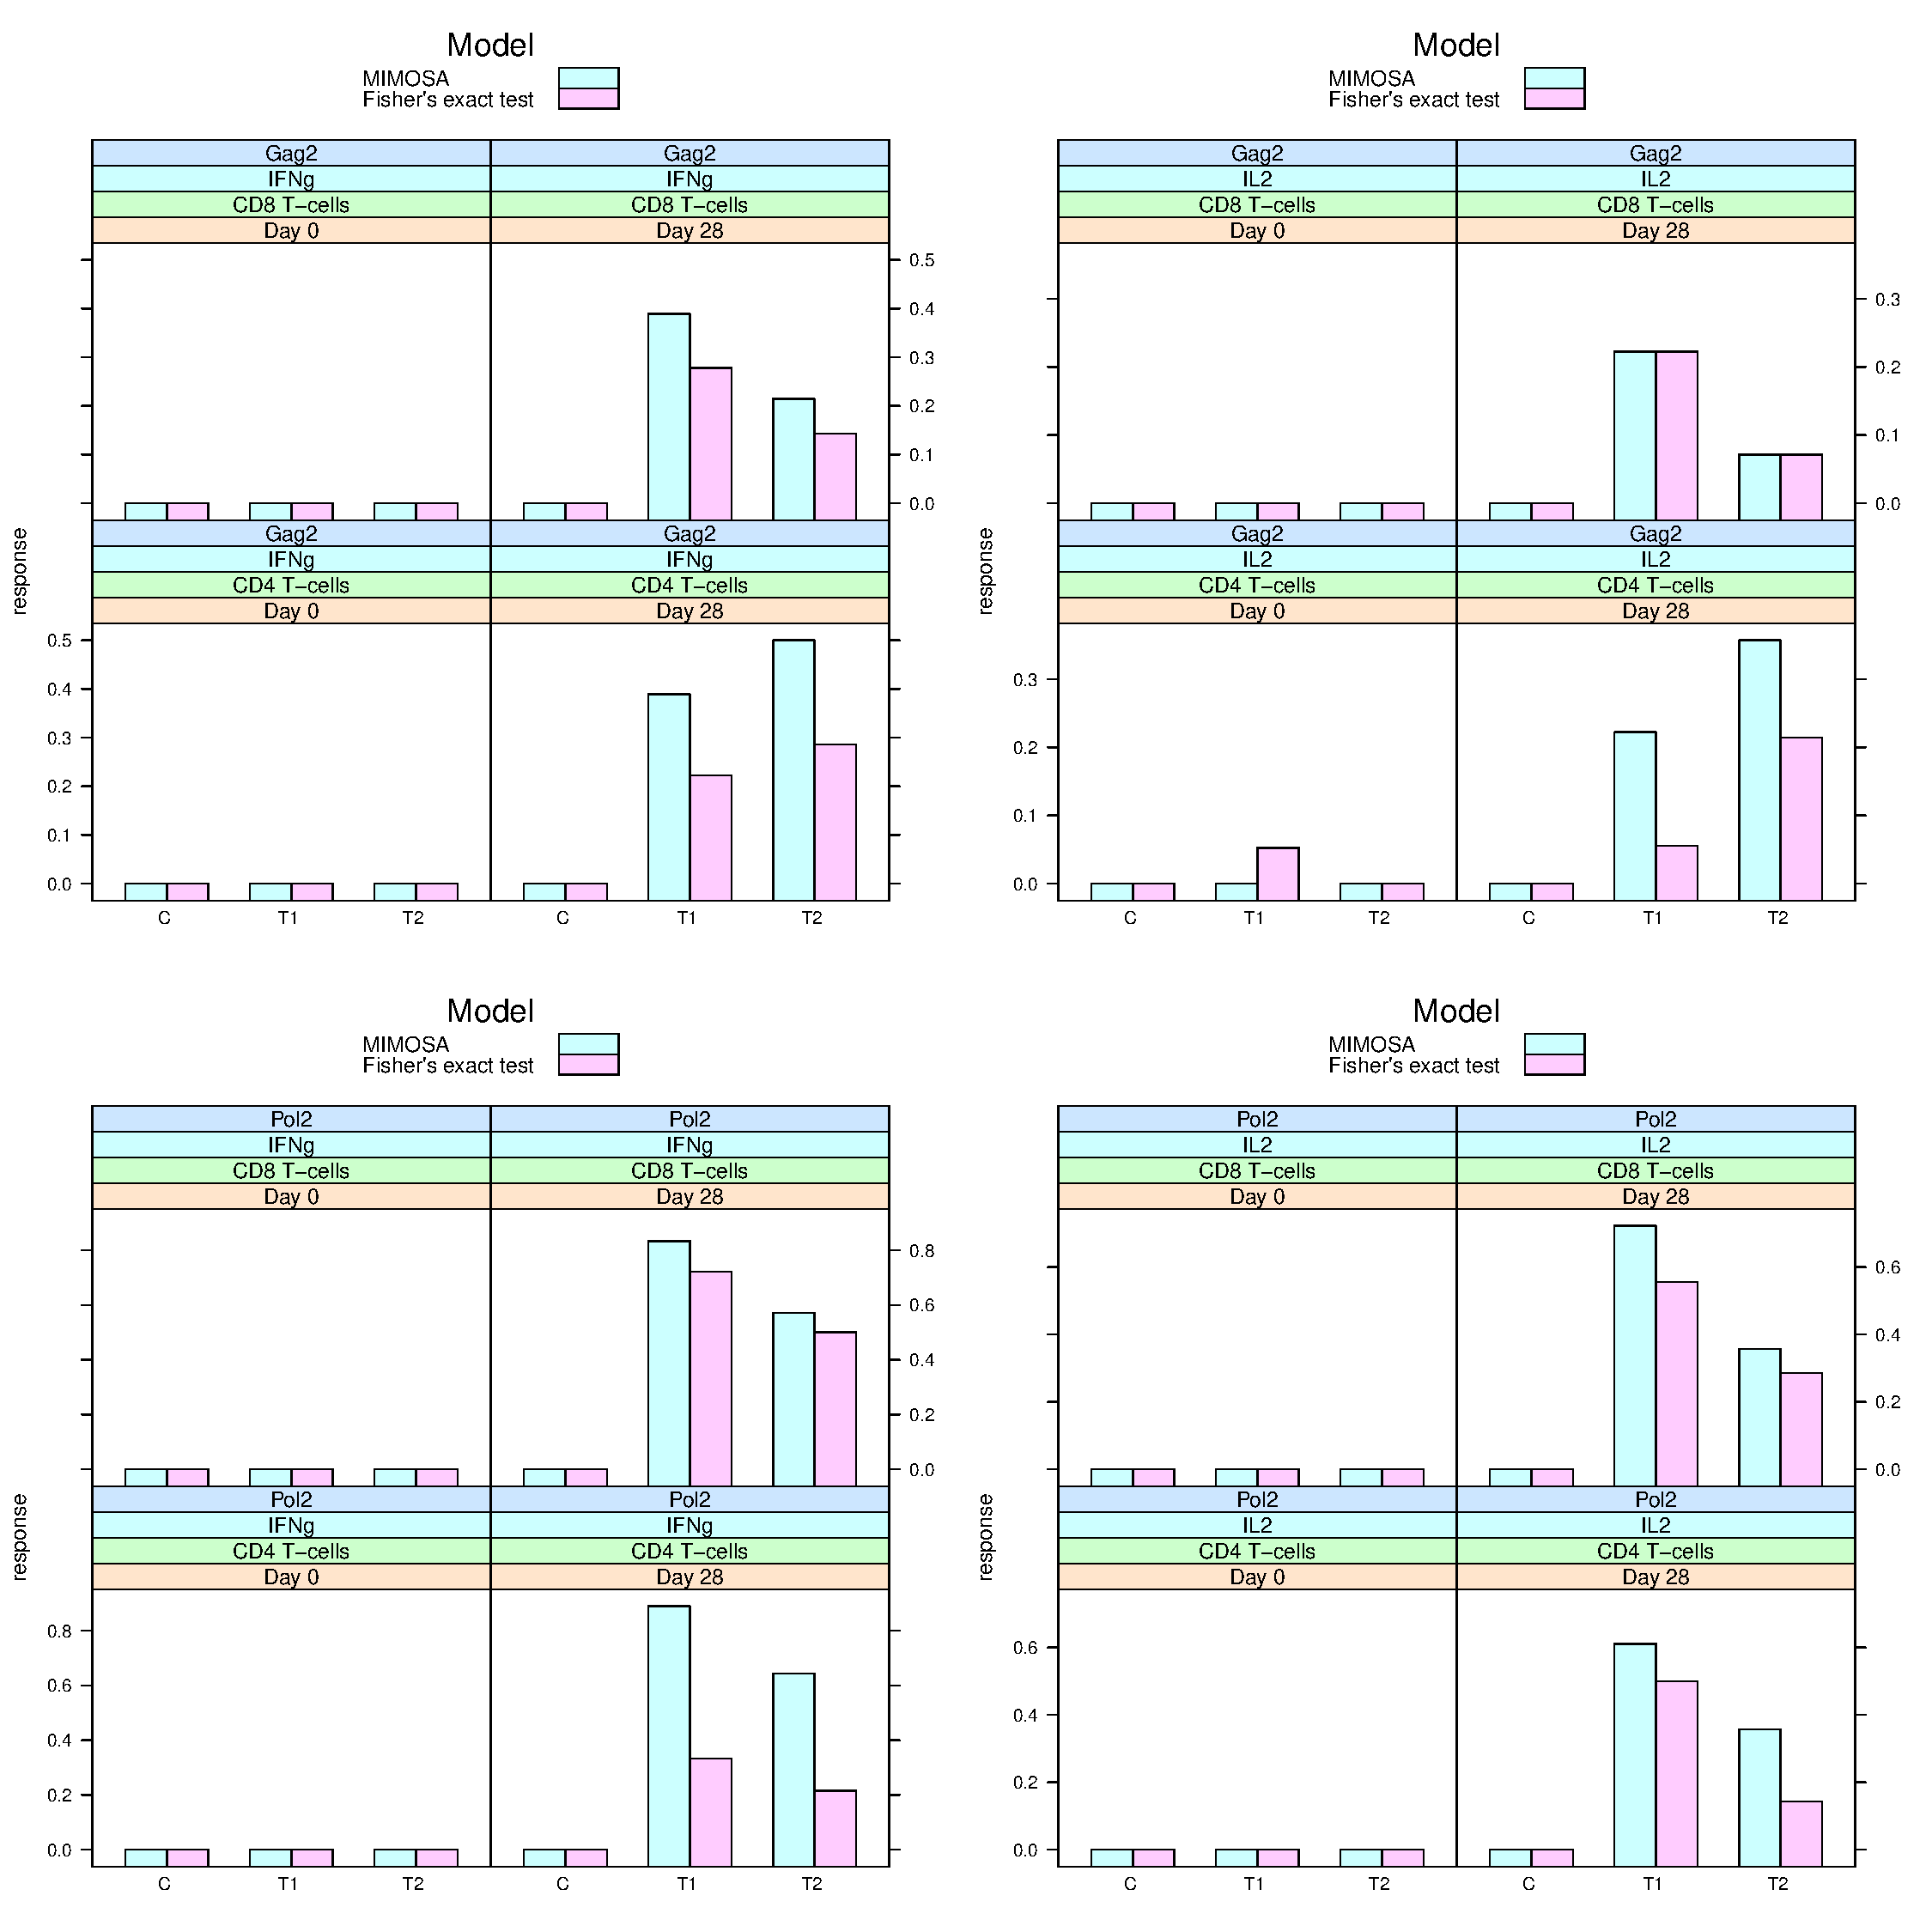
\includegraphics[width=6in]{Figures/PositivityRates} 
   \caption{Comparison of MIMOSA and Fisher's exact test for calling responders in ICS data. Response rates for IL2 and IFNg cytokine positivity in Gag2 and Pol2 stimulated samples at days 0 and 28 in the CD4 and CD8 T--cell subpopulations of the HVTN054 ICS data. In the treatment groups, response rates for the MIMOSA model are greater than or equal to those for Fisher's exact test at day 28 but are equal (and zero) at day 0 as expected. In the control groups, response rates are equal (and zero) between Fisher's exact test and the MIMOSA model at day 0 and at day 28, as expected.}
   \label{fig:positivityrates}
\end{figure}

\begin{figure}[htbp] %  figure placement: here, top, bottom, or page
   \centering
   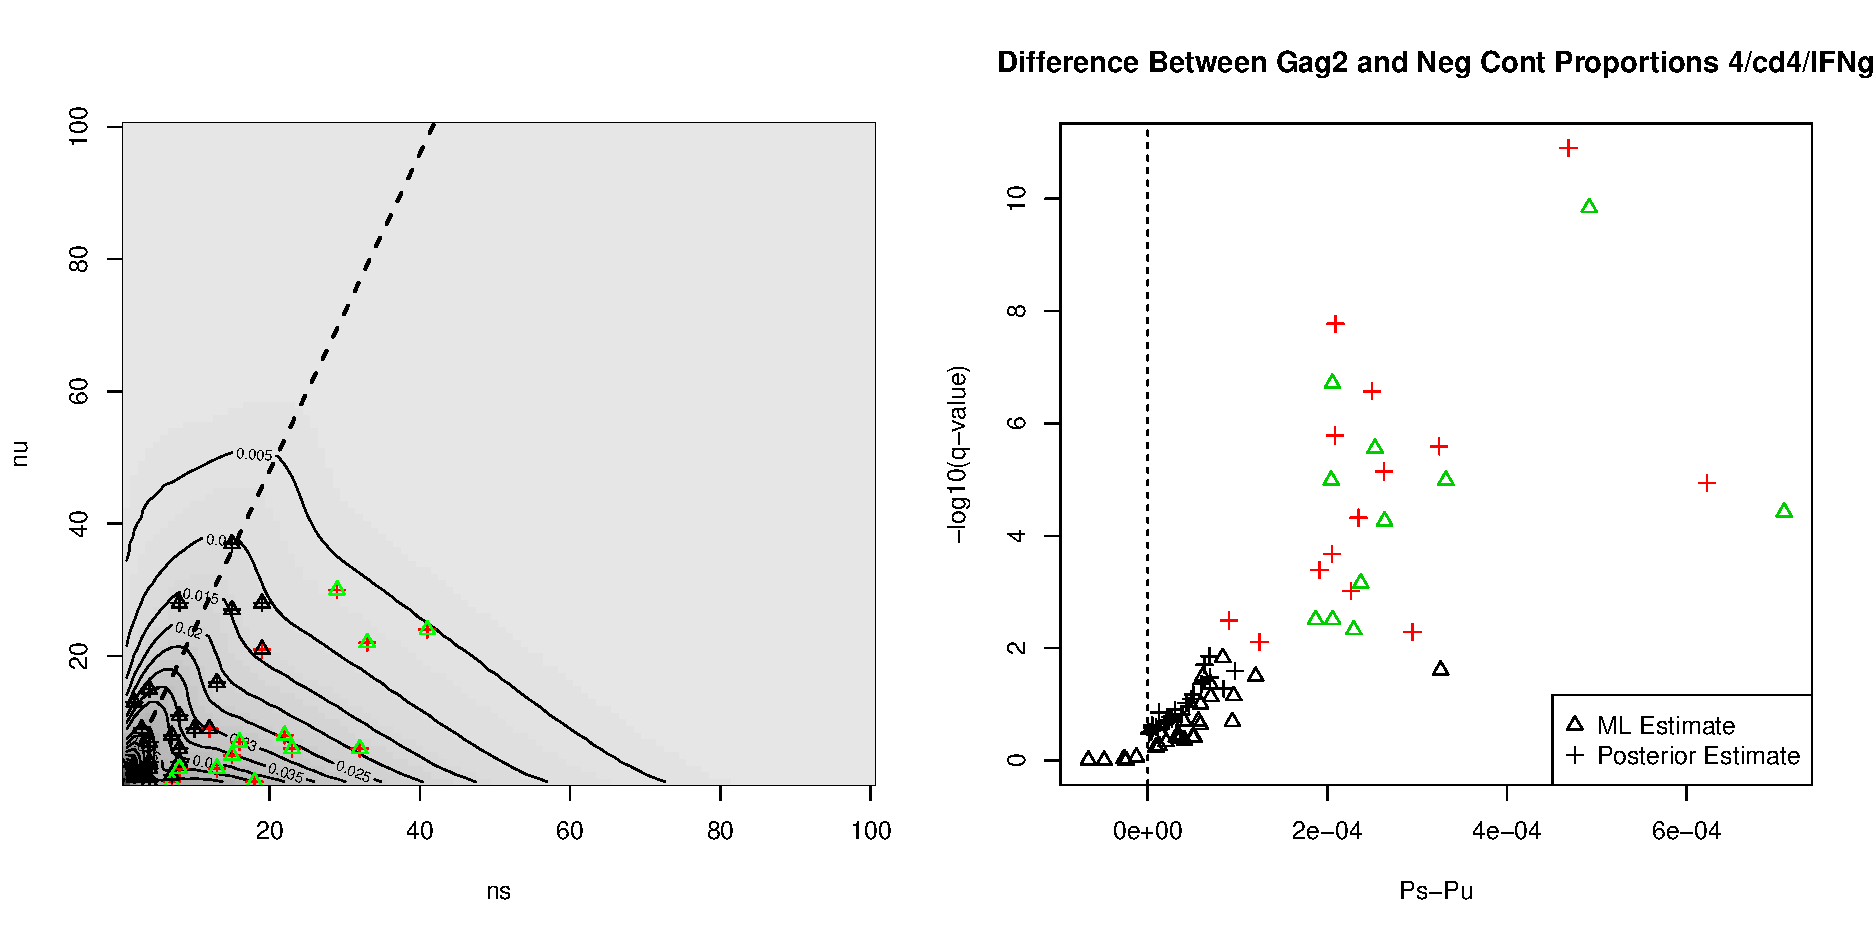
\includegraphics[width=6in]{Figures/HVTN054LikelihoodAndVolcanoplots} 
   \caption{Likelihood surface and volcano plot for IFNg producing, CD4+ T-cells in Gag2 stimulated vs control samples on day 28. A significant difference between control and stimulated samples is called at the 1\% FDR threshold (red) for the Beta--binomial model, and at 1\% for FDR adjusted p--values from Fisher's exact test (green). The likelihood surface shows the observed counts from stimulated and unstimulated samples. The volcano plot shows the difference between the proportion of cytokine positive cells in the stimulated and unstimulated samples, for the maximum likelihood estimates of the proportions (triangles) and for the MAP estimates (crosses). The effect of shrinking the MAP estimates towards zero can be seen in the volcano plot.}
   \label{fig:icsdata}
\end{figure}


\section*{Discussion}

\section*{Conclusions}

%\renewcommand{\thesection}{S.\arabic{section}}
%\renewcommand{\thesubsection}{\thesection.\arabic{subsection}}
%\todo[inline]{Note that the Supplementary Information section needs corrections to notation and overall}
%\section{Supplementary Information}
%\subsection{Derivation of the Beta--Binomial Model for $p_s=p_u$ and $p_s>p_u$}
%\label{sec:derivation}
%
%We derive the posterior predictive distribution and marginal log--likelihood for the null model ($p_s=p_u$) and the alternative model ($p_s>p_u$) below: patient indices, $i$ on the $\left<N_s,n_s,N_u,n_u\right>$ are omitted for clarity. 
%For model \eqref{eq:null}, ($p_s=p_u, \alpha_s=\alpha_u, \beta_s=\beta_u$), the posterior predictive distribution of the data given the model is:
% \begin{align}
% 	\mathrm{Pr}(y_i|\alpha_u,\beta_u) &= \int\limits_{p_u=0}\limits^{1} \mathrm{Pr}(y_i,p_u|\alpha_u,\beta_u)dp_u\\
%	&=\int\limits_{p_u=0}\limits^{1} \mathrm{Pr}(y_i|p_u)\mathrm{Pr}(p_u|\alpha_u,\beta_u)dp_u\\
%	\begin{split}
%		=\int\limits_{p_u=0}\limits^{1}\binom{N_s+n_s}{n_s}p_u^{n_s}(1-p_u)^{N_s}\binom{N_u+n_u}{n_u}p_u^{n_u}(1-p_u)^{N_u}\cdot \\ 
%		\frac{1}{\mathrm{B}(\alpha_u,\beta_u)}p_u^{\alpha_u-1}(1-p_u)^{\beta_u-1}dp_u
%	 \end{split}\\
%	 \begin{split}
% 	=\binom{N_s+n_s}{n_s}\binom{N_u+n_u}{n_u}\frac{1}{\mathrm{B}(\alpha_u,\beta_u)}\cdot\\ \int\limits_{p_u=0}\limits^{1}p_u^{n_s+n_u+\alpha_u-1}(1-p_u)^{N_s+N_u+\beta_u-1}dp_u
%	\end{split}\\
%	\intertext{The integrand is the kernel of a beta distribution with parameters $\left(n_u+n_s+\alpha_u,N_u+N_s+\beta_u\right)$, giving a closed form expression for the  posterior predictive distribution of model \eqref{eq:null}:}
%	\mathrm{Pr}(y_i|\alpha_u,\beta_u)&=\binom{N_s+n_s}{n_s}\binom{N_u+n_u}{n_u}\frac{\mathrm{B}(n_s+n_u+\alpha_u,N_s+N_u+\beta_u)}{\mathrm{B}(\alpha_u,\beta_u)}\label{eq:model1postsupp}\\
%	\intertext{with marginal log--likelihood:}
%	\begin{split}
%	\mathcal{L}(\alpha_u,\beta_u|\mathbf{y})=\sum_{i=1}^P\left[\log{\binom{N^i_{s}+n^i_{s}}{n^i_{s}}}+\log{\binom{N^i_{u}+n^i_{u}}{n^i_{u}}}+\right.\\
%	\left.\log{\left(\mathrm{B}(n^i_s+n^i_u+\alpha_u,N^i_s+N^i_u+\beta_u)\right)}\right]-P\log\left(\mathrm{B}(\alpha_u,\beta_u)\right)\label{eq:model1MLLsupp}
%	\end{split}
% \end{align} 
% 
%For model \eqref{eq:alternate}, ($p_s>p_u$), the posterior predictive distribution of the data given the model is:
%\begin{align}
% 	\mathrm{Pr}(y_i|\alpha_u,\beta_u,\alpha_s,\beta_s) &= \int\limits_{p_u=0}\limits^1\int\limits_{p_s>p_u}\limits^{1} \mathrm{Pr}(y_i,p_u,p_s|\alpha_u,\beta_u,\alpha_s,\beta_s) dp_u  dp_s\label{eq:postpredmodel2}\\
%	\intertext{Assuming independence of stimulated and unstimulated observations in \eqref{eq:postpredmodel2}:} 
%	&=\int\limits_{p_u=0}\limits^{1}\int\limits_{p_s>p_u}\limits^1 \mathrm{Pr}(n_s|p_s)\mathrm{Pr}(n_u|p_u)\mathrm{Pr}(p_u|\alpha_u,\beta_u)\mathrm{Pr}(p_s|\alpha_s,\beta_s)dp_u dp_s\\
%		&=\int\limits_{p_u=0}\limits^{1}\mathrm{Pr}(n_u|p_u)\mathrm{Pr}(p_u|\alpha_u,\beta_u)dp_u \int\limits_{p_s>p_u}\limits^1 \mathrm{Pr}(n_s|p_s)\mathrm{Pr}(p_s|\alpha_s,\beta_s)dp_s\\
%		\begin{split}
%	=\int\limits_{p_u=0}\limits^{1}\left[ \binom{N_u+n_u}{n_u}p_u^{n_u}(1-p_u)^{N_u} \frac{1}{\mathrm{B}(\alpha_u,\beta_u)}p_u^{\alpha_u-1}(1-p_u)^{\beta_u-1}d p_u\right]\cdot \\ \int\limits_{p_s>p_u}\limits^{1}\left[ \binom{N_s+n_s}{n_s}p_s^{n_s}(1-p_s)^{N_s} \frac{1}{\mathrm{B}(\alpha_s,\beta_s)}p_s^{\alpha_s-1}(1-p_s)^{\beta_s-1}d p_s\right]
%	\end{split}\\
%	\begin{split}
%	 =\binom{N_u+n_u}{n_u} \binom{N_s+n_s}{n_s}\frac{1}{\mathrm{B}(\alpha_u,\beta_u)}\frac{1}{\mathrm{B}(\alpha_s,\beta_s)}\cdot\\
%	 \int\limits_{p_u=0}\limits^{1}\left[p_u^{n_u+\alpha_u-1}(1-p_u)^{N_u+\beta_u-1} d p_u\right]\int\limits_{p_s>p_u}\limits^{1}\left[p_s^{n_s+\alpha_s-1}(1-p_s)^{N_s+\beta_s-1}d p_s\right]
%	\end{split}
%	\end{align}
%	\begin{align}
%	\begin{split}
%	 =\binom{N_u+n_u}{n_u} \binom{N_s+n_s}{n_s}\frac{1}{\mathrm{B}(\alpha_u,\beta_u)}\frac{1}{\mathrm{B}(\alpha_s,\beta_s)}\cdot\\
%	 \int\limits_{p_u=0}\limits^{1}\left[p_u^{n_u+\alpha_u-1}(1-p_u)^{N_u+\beta_u-1}d p_u \right]\left(1-\int\limits^{p_u}\limits_{p_s=0}\left[p_s^{n_s+\alpha_s-1}(1-p_s)^{N_s+\beta_s-1}d p_s\right]\right)
%	\end{split}
%	\intertext{The second integral can be expressed as the CDF of the beta distribution, also known as the regularized incomplete beta function, $\mathrm{I}_x(\alpha,\beta)$}
%	\begin{split}
%	 =\binom{N_u+n_u}{n_u} \binom{N_s+n_s}{n_s}\frac{1}{\mathrm{B}(\alpha_u,\beta_u)}\frac{\mathrm{B}(n_s+\alpha_s,N_s+\beta_s)}{\mathrm{B}(\alpha_s,\beta_s)}\cdot\\
%	 \int\limits_{p_u=0}\limits^{1}\left[p_u^{n_u+\alpha_u-1}(1-p_u)^{N_u+\beta_u-1} \right]\left(1-\mathrm{I_{p_s}}(n_s+\alpha_s,N_s+\beta_s)\right)d p_u
%	\end{split}\\
%	\intertext{giving the posterior predictive distribution of model \eqref{eq:alternate}}
%	\begin{split}
%		 =\binom{N_u+n_u}{n_u} \binom{N_s+n_s}{n_s}\frac{\mathrm{B}(n_u+\alpha_u,N_u+\beta_u)}{\mathrm{B}(\alpha_u,\beta_u)}\frac{\mathrm{B}(n_s+\alpha_s,N_s+\beta_s)}{\mathrm{B}(\alpha_s,\beta_s)}\cdot\\
%	 \int\limits_{p_u=0}\limits^{1}\left[\frac{1}{\mathrm{B}(n_u+\alpha_u,N_u+\beta_u)}p_u^{n_u+\alpha_u-1}(1-p_u)^{N_u+\beta_u-1} \right]\left(1-\mathrm{I_{p_u}}(n_s+\alpha_s,N_s+\beta_s)\right)d p_u\label{eq:model2postsupp}
%	\end{split}
%\end{align}
%The integral in equation~\eqref{eq:model2postsupp} is computed numerically. The marginal log--likelihood of model~\eqref{eq:alternate} is then:
%\begin{equation}
%		 \begin{split}
%		 \mathcal{L}(\alpha_s,\alpha_u,\beta_s,\beta_u|\mathbf{y})=-P\log\left(\mathrm{B}(\alpha_u,\beta_u)\right)-P\log\left(\mathrm{B}+(\alpha_s,\beta_s)\right)+\\ \sum_{i=0}^P\left\{\log\binom{N^i_u+n^i_u}{n^i_u}+ \log\binom{N^i_s+n^i_s}{n^i_s}+ \log\left(\mathrm{B}(n^i_u+\alpha_u,N^i_u+\beta_u)\right)+ \log\left(\mathrm{B}(n^i_s+\alpha_s,N^i_s+\beta_s)\right)+\right. \\ \left. \log\left(\hspace{1em}\int\limits_{p_u=0}\limits^{1}\left[\frac{1}{\mathrm{B}(n^i_u+\alpha_u,N^i_u+\beta_u)}p_u^{n^i_u+\alpha_u-1}(1-p_u)^{N^i_u+\beta_u-1} \right]\left(1-\mathrm{I_{p_u}}(n^i_s+\alpha_s,N^i_s+\beta_s)\right)d p_u\right)\right\}\label{eq:model2MLLsupp}
%\end{split}
%\end{equation}
%\subsection{The Beta-Binomial Mixture Model}
%For a given stimulation, not all individuals are expected to exhibit an immune response to that stimulation. Therefore, for a set of ICS data, any single observation, ($n^i_s,n^i_u$) could either be derived from model~\eqref{eq:null}, or from model~\eqref{eq:alternate}. We model this situation explicitly using a mixture--model framework.
\clearpage
\bibliographystyle{unsrtnat}
\bibliography{MIMOSA}

\end{document}  
